\newcommand{\streamlinecomment}[1]{}

This chapter describes the \cgal's 2D streamline placement package.
Basic definitions and notions are given in section \ref{Section_2D_Streamlines_Definitions}.
Section \ref{Section_2D_Streamlines_Fundamental_notions} gives a description of the integration process.
Section \ref{Section_2D_Streamlines_Strategy} describes briefly the algorithm.
Section \ref{Section_2D_Streamlines_Implementation} presents the implementation of the package, and
section \ref{Section_2D_Streamlines_Example} gives two examples of using the package.

\begin{figure}[h!]
\begin{ccTexOnly}
\begin{center}
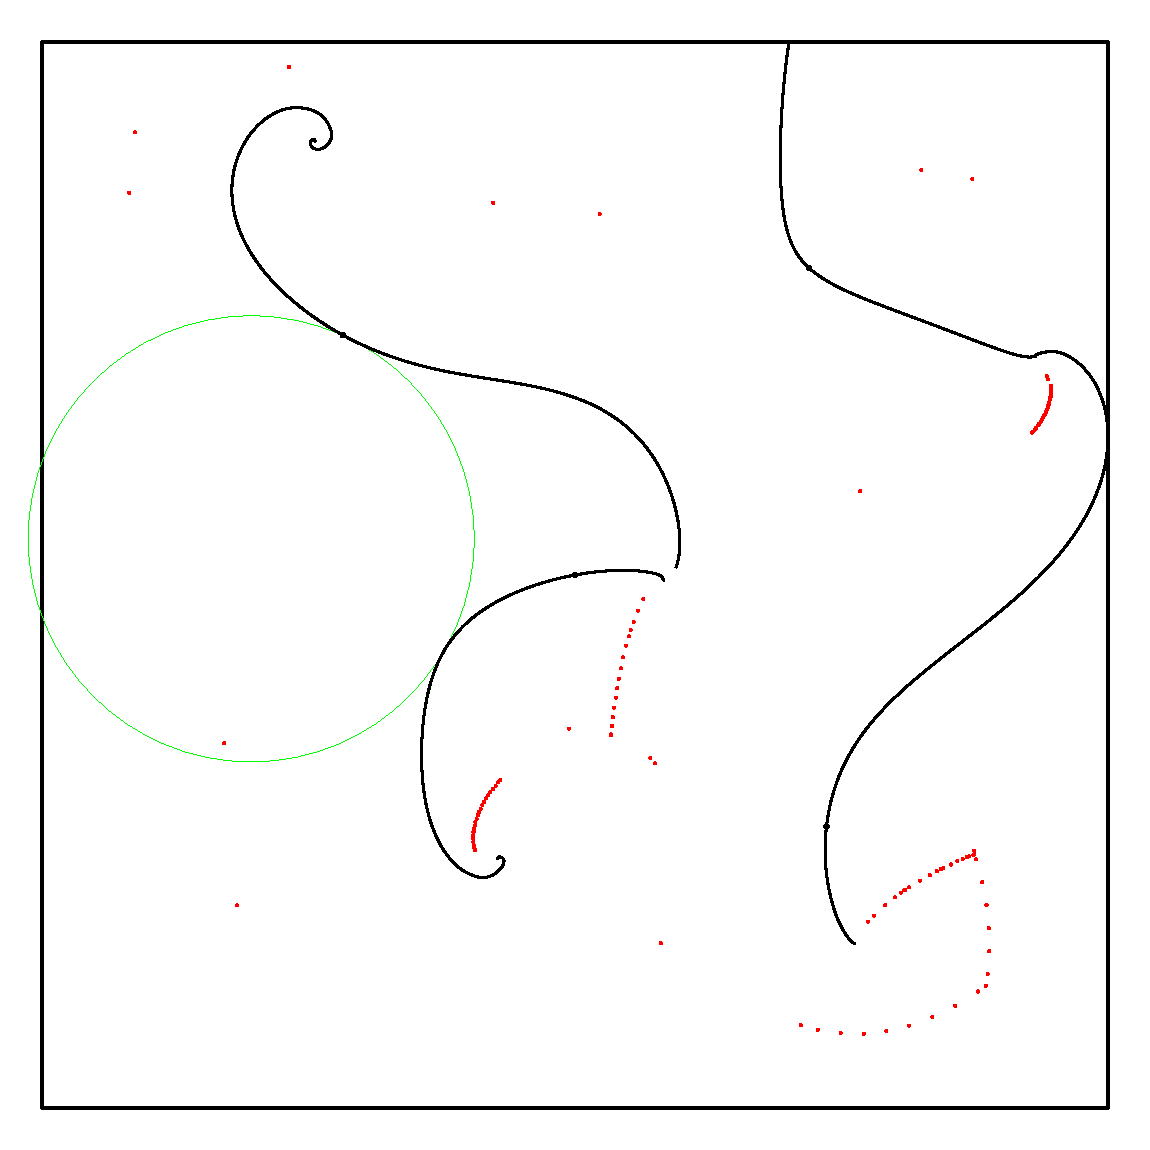
\includegraphics[width=4cm]{Stream_lines_2/1} \hspace*{0.5cm} 
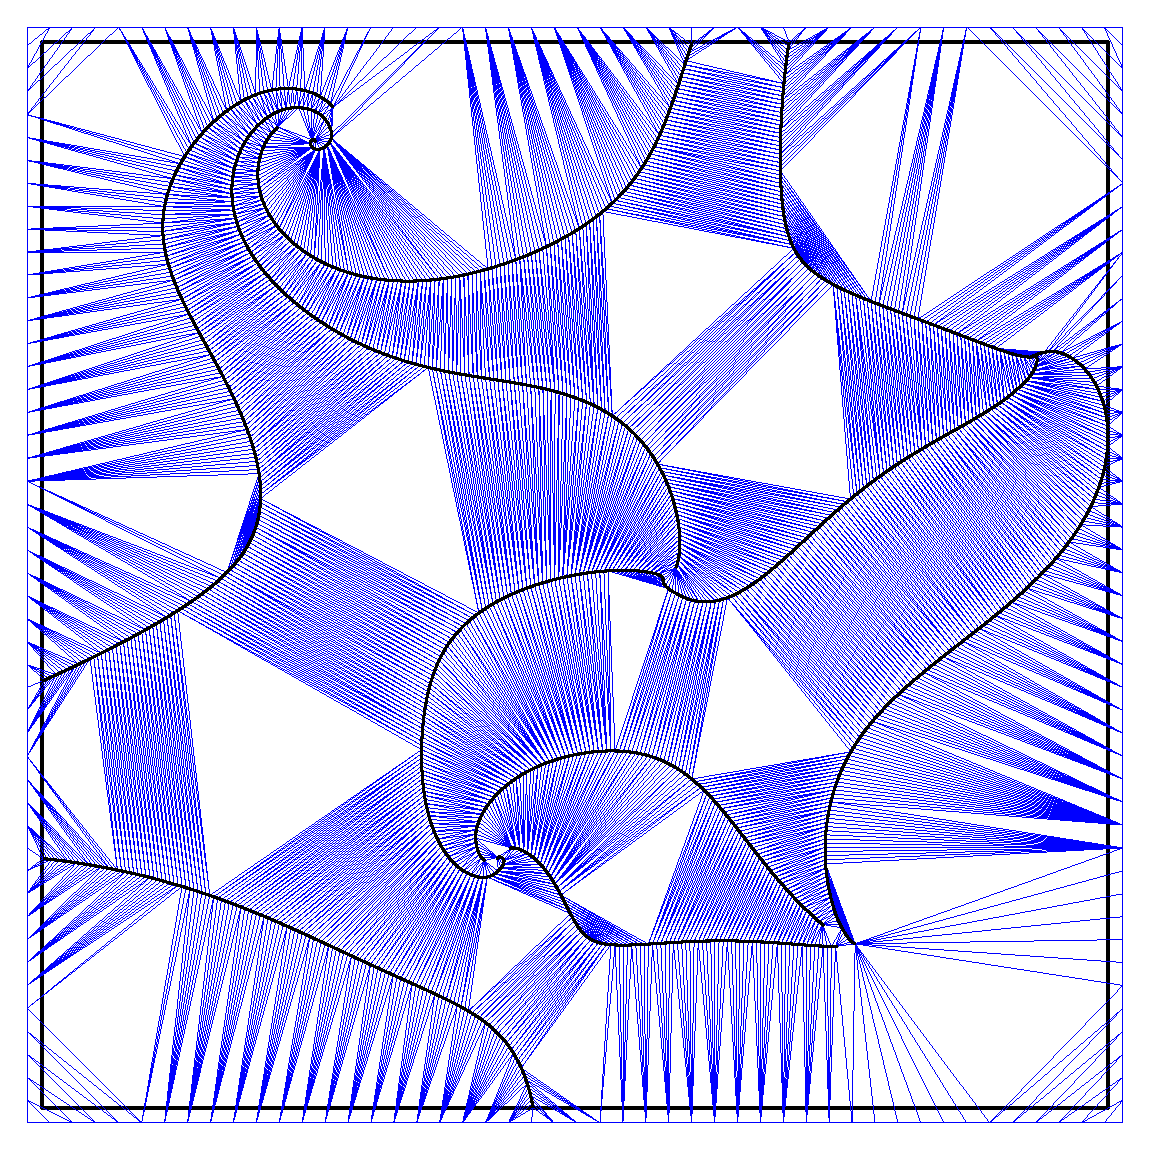
\includegraphics[width=4cm]{Stream_lines_2/2} \hspace*{0.5cm} 
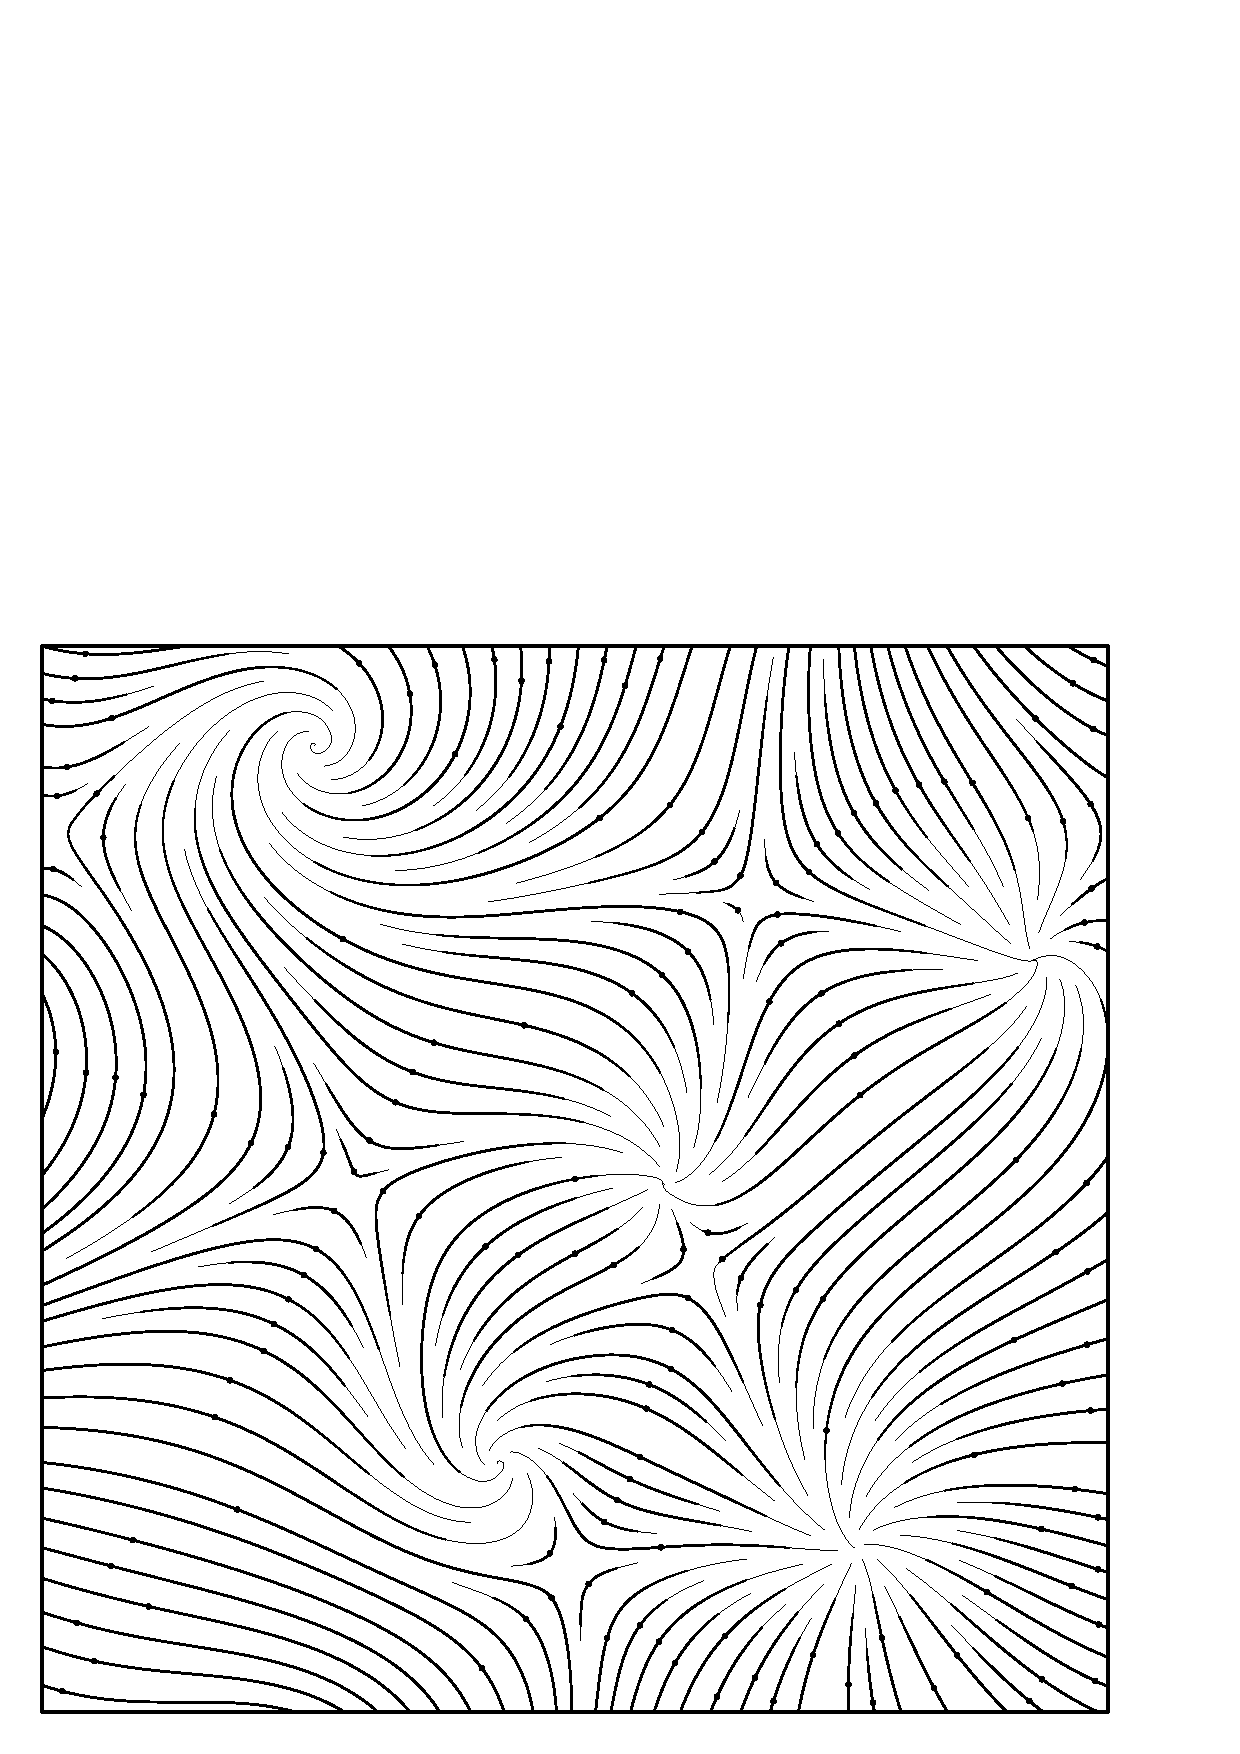
\includegraphics[width=4cm]{Stream_lines_2/3}
\end{center}
\end{ccTexOnly}
\caption{The core idea of the algorithm is to integrate the streamlines from the center of the biggest empty cavities in the domain (left figure). A Delaunay triangulation of all the sample points is used to model the streamlines and the spaces in the domain (middle figure). A typical result is shown in the right figure.}
\label{illustration}
\begin{ccHtmlOnly}
<CENTER>
<img border=0 src="./1.gif" width=300>
<img border=0 src="./2.gif" width=300>
<img border=0 src="./3.gif" width=300>
</CENTER>
\end{ccHtmlOnly}
\end{figure}

\section{Definitions}
\label{Section_2D_Streamlines_Definitions}
In physics, a \ccc{field} is an assignment of a quantity to every point in
space. For example, one can speak of a gravitational field, which assigns a
gravitational potential to each point in space.\\
Vector and direction fields are commonly used for modeling physical phenomena,
where a direction and magnitude,
or a vector is assigned to each point inside a domain (such as the magnitude and
direction of the force at each point in a magnetic field).\\
Streamlines are very important tools for visualizing those entities. A
\ccc{streamline} is a curve everywhere tangent to the field. In practice, 
a streamline is often represented as a polyline iteratively elongated by 
bidirectional numerical integration started from a \ccc{seed point}, until 
it comes close to another streamline (according to a specified distance called 
the \ccc{the separating distance}), hits the domain boundary, reaches a 
critical point or generates a closed path.\\
A \ccc{valid} placement of streamlines consists of saturating the domain with a set of tangential streamlines  in accordance with a specified \ccc{density}, determined by the \ccc{separating distance} between the streamlines.

\section{Fundamental notions}
\label{Section_2D_Streamlines_Fundamental_notions}
A streamline can be considered as the path traced by an imaginary massless particle dropped into a steady fluid flow described by the field. The construction of this path consists in the resolution of an ordinary differential equation for different successive time intervals. In this way, we obtain series of points $p_k, 0<k<n$ that allows the visualization of the streamline.
This equation is defined as follows : $$\frac{dp}{dt} = v(p(t)), p(0) = p_0$$ where \ccc{p(t)} is the position of the particle at time \ccc{t}, \ccc{v} is a function that gives the vector value in each point in the domain (even by interpolation), and $p_0$ is the initial position.
The position after a given interval $\Delta t$ is given by : $$p(t + \Delta t) = p(t) + \int_t^{t+\Delta t} v(p(t)) dt$$
Several numeric methods has been proposed to solve this equation, in this package, two methods are implemented : Euler algorithm, and Second Order Runge Kutta algorithm.

\subsection{Euler integrator}

\begin{figure}[h!]
\begin{ccTexOnly}
\begin{center}
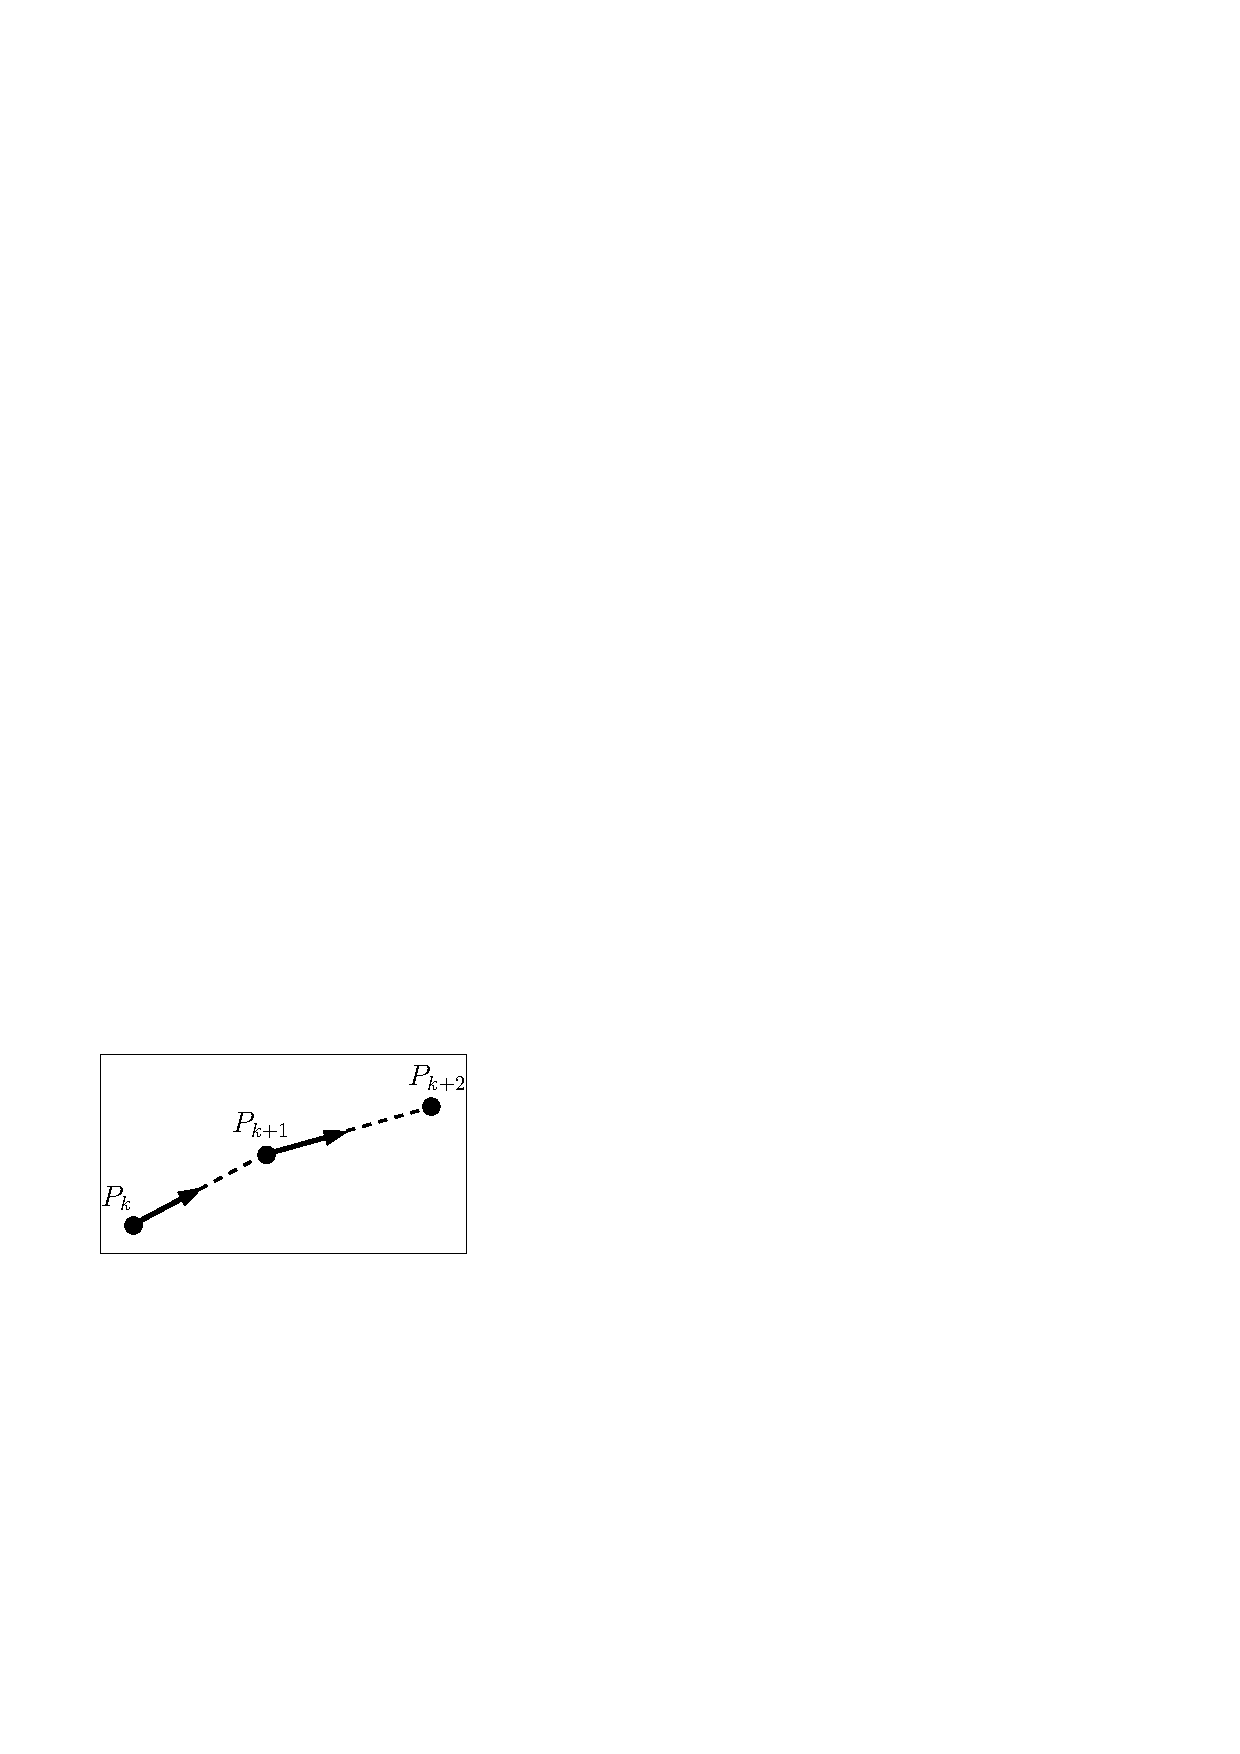
\includegraphics[width=4cm]{Stream_lines_2/euler_integrator}
\end{center}
\end{ccTexOnly}
\caption{Euler integrator.
\label{euler_fig}}
\begin{ccHtmlOnly}
<CENTER>
<img border=0 src="./euler_integrator.gif" width=175>
</CENTER>
\end{ccHtmlOnly}
\end{figure}

This algorithm approximates the point computation by this formula $$p_{k+1} = p_k + hv(p_k)$$ where \ccc{h} specifies the \ccc{integration step} (see~figure~\ref{euler_fig}). The integration can be done forward and backward by specifying a negative integration step \ccc{h}. The streamline is then constructed by successive integration from a seed point forward and backward.

\subsection{Second Order Runge Kutta integrator}

\begin{figure}[h!]
\begin{ccTexOnly}
\begin{center}
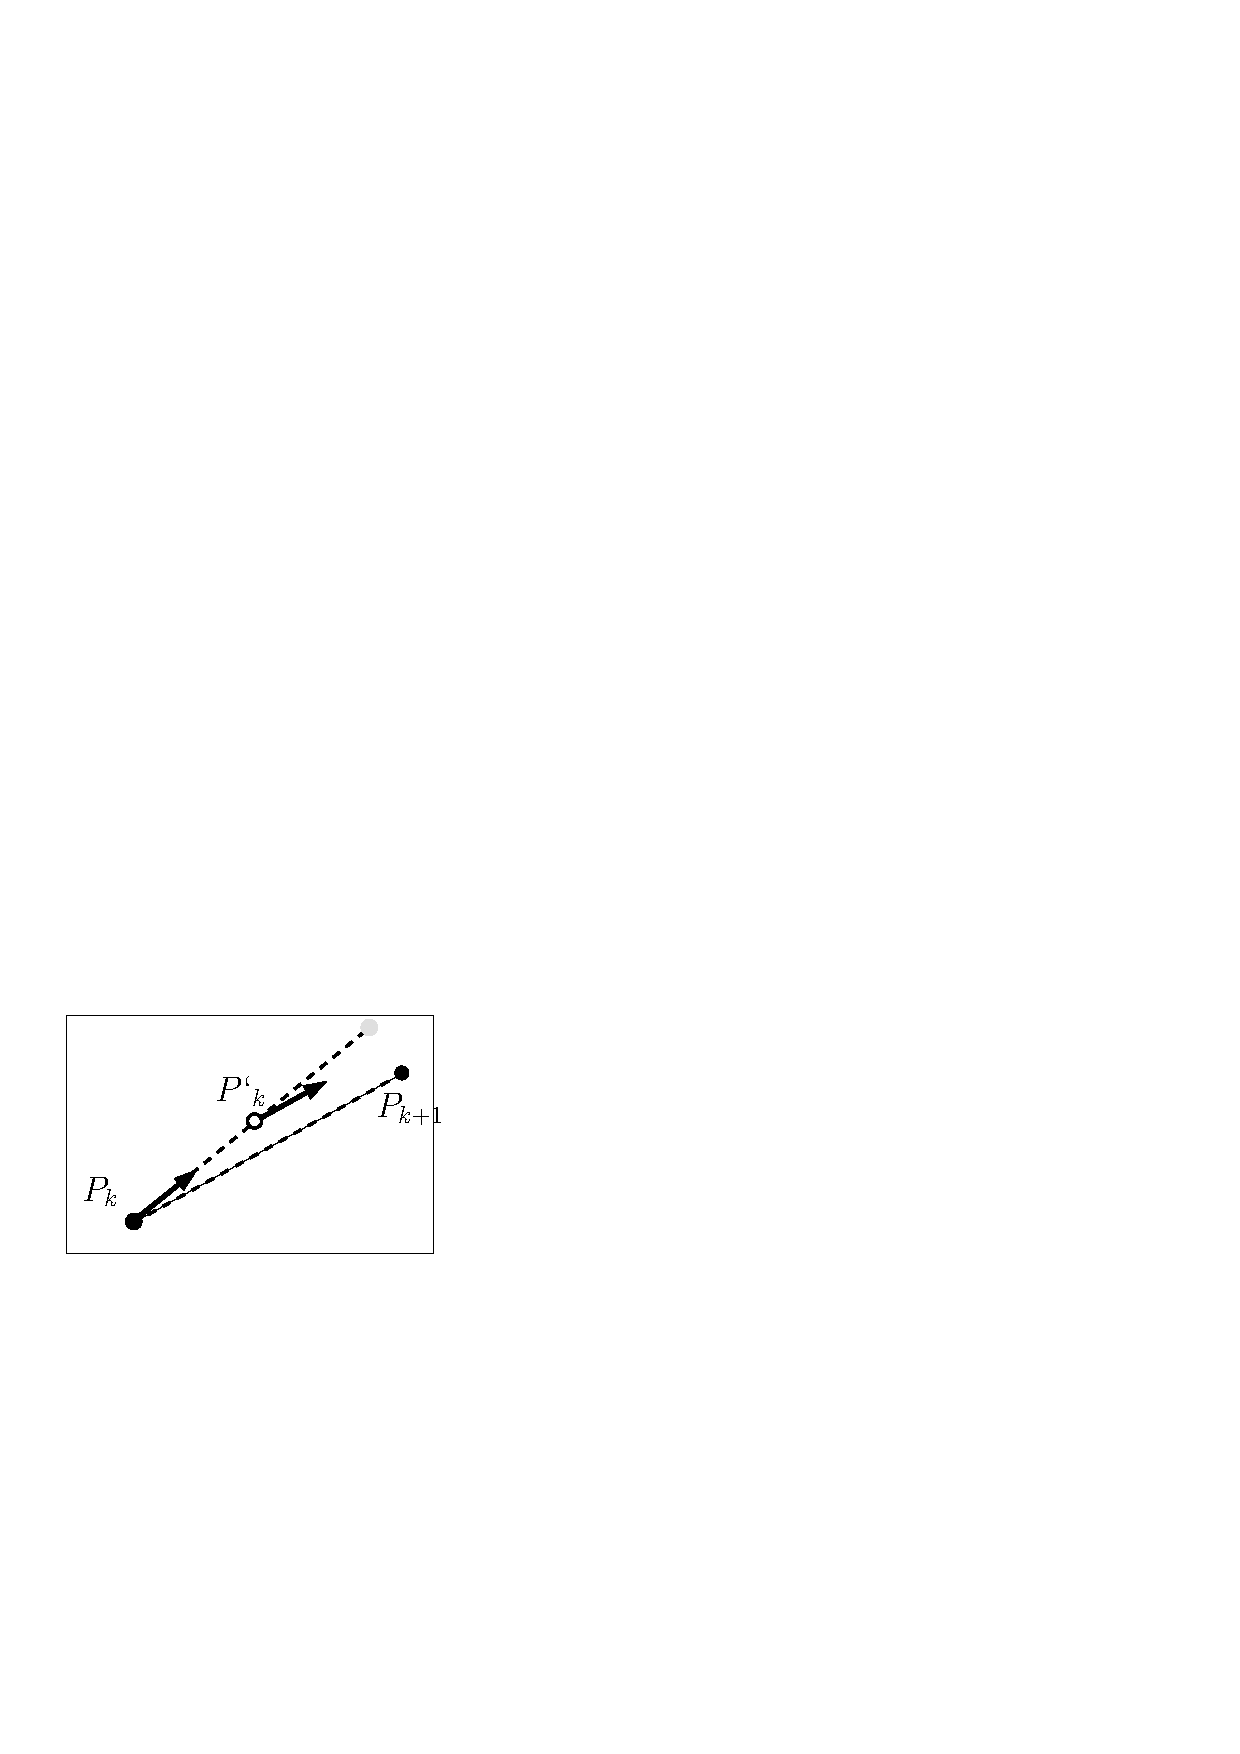
\includegraphics[width=4cm]{Stream_lines_2/runge_kutta_integrator}
\end{center}
\end{ccTexOnly}
\caption{Runge-kutta second order integrator (The empty circle represents the intermediate point, and the gray disk represents the Euler integrated point).
\label{runge_kutta_fig}}
\begin{ccHtmlOnly}
<CENTER>
<img border=0 src="./runge_kutta_integrator.gif" width=175>
</CENTER>
\end{ccHtmlOnly}
\end{figure}

This method introduce an intermediate point \ccc{p'} to have more precision in the computation (see~figure~\ref{runge_kutta_fig})

$$\{ \begin{array}{ccc} p`_k & = & p_k + \frac{1}{2}hv(p_k) \\ p_{k+1} & = & p_k + hv(p`_k) \end{array}$$

See~\cite{cgal:ptvf-nrcpp-02} for further information.


\section{Farthest point seeding strategy}
\label{Section_2D_Streamlines_Strategy}
The algorithm implemented in this package~\cite{cgal:mad-fpsep-05} consists of
placing one streamline at
a time by numerical integration starting at the furthest away from all
previously placed streamlines.\\The input of our algorithm is given by
(i) a flow field, (ii) a \textit{density} specified either globally, by the
inverse of the ideal spacing distance, or locally by a density field, and (iii)
a \textit{saturation} ratio over the desired spacing required to trigger the
seeding of a new streamline.\\The input flow field is given by a discrete set of
vectors or directions sampled within a domain, associated with an interpolation
scheme (\textit{e.g.} bilinear interpolation over a regular grid, or natural
neighbor interpolation over an irregular point set to
allow for an evaluation at each point coordinate within the domain).\\The
\textit{output} is a streamline placement, represented as a list of streamlines.
The core idea of our algorithm consists of placing one streamline at a time by
numerical integration seeded at the farthest point from all previously placed
streamlines.\\The streamlines are approximated by polylines, whose points are
inserted in a 2D Delaunay triangulation. The empty circumscribed circles of the
Delaunay triangles provide us with a good approximation of the cavities in the
domain.\\After each streamline integration, all incident triangles which
circumcircle diameter is larger (within the saturation ratio) than the desired
spacing distance are pushed to a priority queue sorted by the triangle
circumcircle diameter. To start each new streamline integration, the triangle
with largest circumcircle diameter (and hence the biggest cavity) is popped out
of the queue. We first test if it is still a valid triangle of the
triangulation, since it could have been destroyed by a streamline previously
added to the triangulation. If it is not, we pop another triangle out of the
queue. If it is, we use the center of its circumcircle as seed point to
integrate a new streamline.\\Our algorithm terminates when the priority queue is empty. The size
of the biggest cavity being monotonically decreasing, our algorithm guarantees
the domain saturation.

\section{Implementation}
\label{Section_2D_Streamlines_Implementation}
Streamlines are represented as polylines, and are obtained by iterative
integration from the seed point. The computation is processed via a list of
Delaunay triangulation vertices.\\To implement the triangular grid, the \cgal\
\ccc{Delaunay_triangulation_2} class is used. The priority queue used to store
candidate seed
points is taken from the Standard Template Library~\cite{cgal:sgcsi-stlpg-97}.

\section{Examples}
\label{Section_2D_Streamlines_Example}
The first example illustrates the generation of a 2D streamline placement from a 
vector field defined on a regular grid.
\ccIncludeExampleCode{Stream_lines_2/stl_regular_field.C}
The second example depicts the generation of a streamline placement from a vector
field defined on a triangular grid.
\ccIncludeExampleCode{Stream_lines_2/stl_triangular_field.C}
